\documentclass[12pt,a4paper]{report}
\usepackage[top=2.5cm,bottom=2.5cm,left=1.5cm,right=1.5cm]{geometry}
\usepackage[rightcaption]{sidecap}
\usepackage{graphicx} %package to manage images
\graphicspath{ {Images/ }}
\usepackage{hyperref}
\usepackage{cmap}
\usepackage{graphicx}
\usepackage[english]{babel}
\usepackage[utf8]{inputenc}
\usepackage[T1]{fontenc}
%\usepackage{lmodern}
\usepackage{ragged2e}
\usepackage{amssymb}
\usepackage{amsmath}

\usepackage{amsthm}
\newtheorem{veta}{Veta}[section]
\newtheorem{lema}[veta]{Lema}
\theoremstyle{definition}
\newtheorem{definicia}{Definícia}[chapter]
\theoremstyle{remark}
\newtheorem*{poznamka}{Poznámka}

\usepackage{setspace}
\onehalfspacing

\begin{document}

%\includepdf{zadanie.pdf}

%%% DEFINÍCIE NÁZVOV
\def\nazov{Skeleton tracking with camera and set of IMUs}
\def\autorT{Bc. Tomáš Sláma }
\def\fakulta{FACULTY OF MATHEMATICS, PHYSICS AND INFORMATICS}
\def\univerzita{COMENIUS UNIVERSITY IN BRATISLAVA}
\def\mesto{Bratislava}
\def\typprace{Diploma thesis}
\def\rok{2018}
\def\bodky{.............................}
%%% OBAL
\thispagestyle{empty}
\begin{center}
\textsc{\LARGE\univerzita}\\
\bigskip\textsc{\LARGE\fakulta}\\
\vfill\textsc{\Huge\nazov}\\
\medskip{\Large\typprace}\\
\vfill{\large\rok\hfill\autorT \\ }
\end{center}

\newpage

%%% DEFINÍCIE NÁZVOV
\def\nazov{Skeleton tracking with Camera and set of IMUs }
\def\autorT{Bc. Tomáš Sláma }
\def\fakulta{FACULTY OF MATHEMATICS, PHYSICS AND INFORMATICS}
\def\univerzita{COMENIUS UNIVERSITY IN BRATISLAVA}
\def\mesto{Bratislava}
\def\typprace{Diploma thesis}
\def\rok{2018}
\def\program{Applied informatics}
\def\odbor{2511 Applied informatics}
\def\pracovisko{Department of applied informatics}
\def\skolitel{RNDr. Martin Madaras, PhD.}

%%% OBAL vnutorny
\thispagestyle{empty}
\begin{center}
\textsc{\LARGE\univerzita}\\
\bigskip\textsc{\LARGE\fakulta}\\
\vfill\textsc{\Huge\nazov}\\
\medskip{\Large\typprace}\\ 
\vfill{
\flushleft\textsc{Study program:\ \ \program}
\flushleft\textsc{Branch of study:\ \ \odbor}
\flushleft\textsc{Department:\ \ \pracovisko}
\flushleft\textsc{Supervisor: \ \ \skolitel}  \hfill \break}
\\
\large\mesto,\ \rok\hfill\autorT \\ 
\end{center}

\newpage

% cestne prehlasenie
\thispagestyle{empty}
\textbf{\Huge }\\

I hereby declare that I have written my diploma thesis on my own and I have only used the sources listed in the bibliography. \\
\newline
\newline
\newline
\large\mesto,\ \rok\hfill\bodky 
\flushright\large\ \autorT \\ 
%koniec prehlasenia

\newpage
\thispagestyle{empty}
%zadanie prace
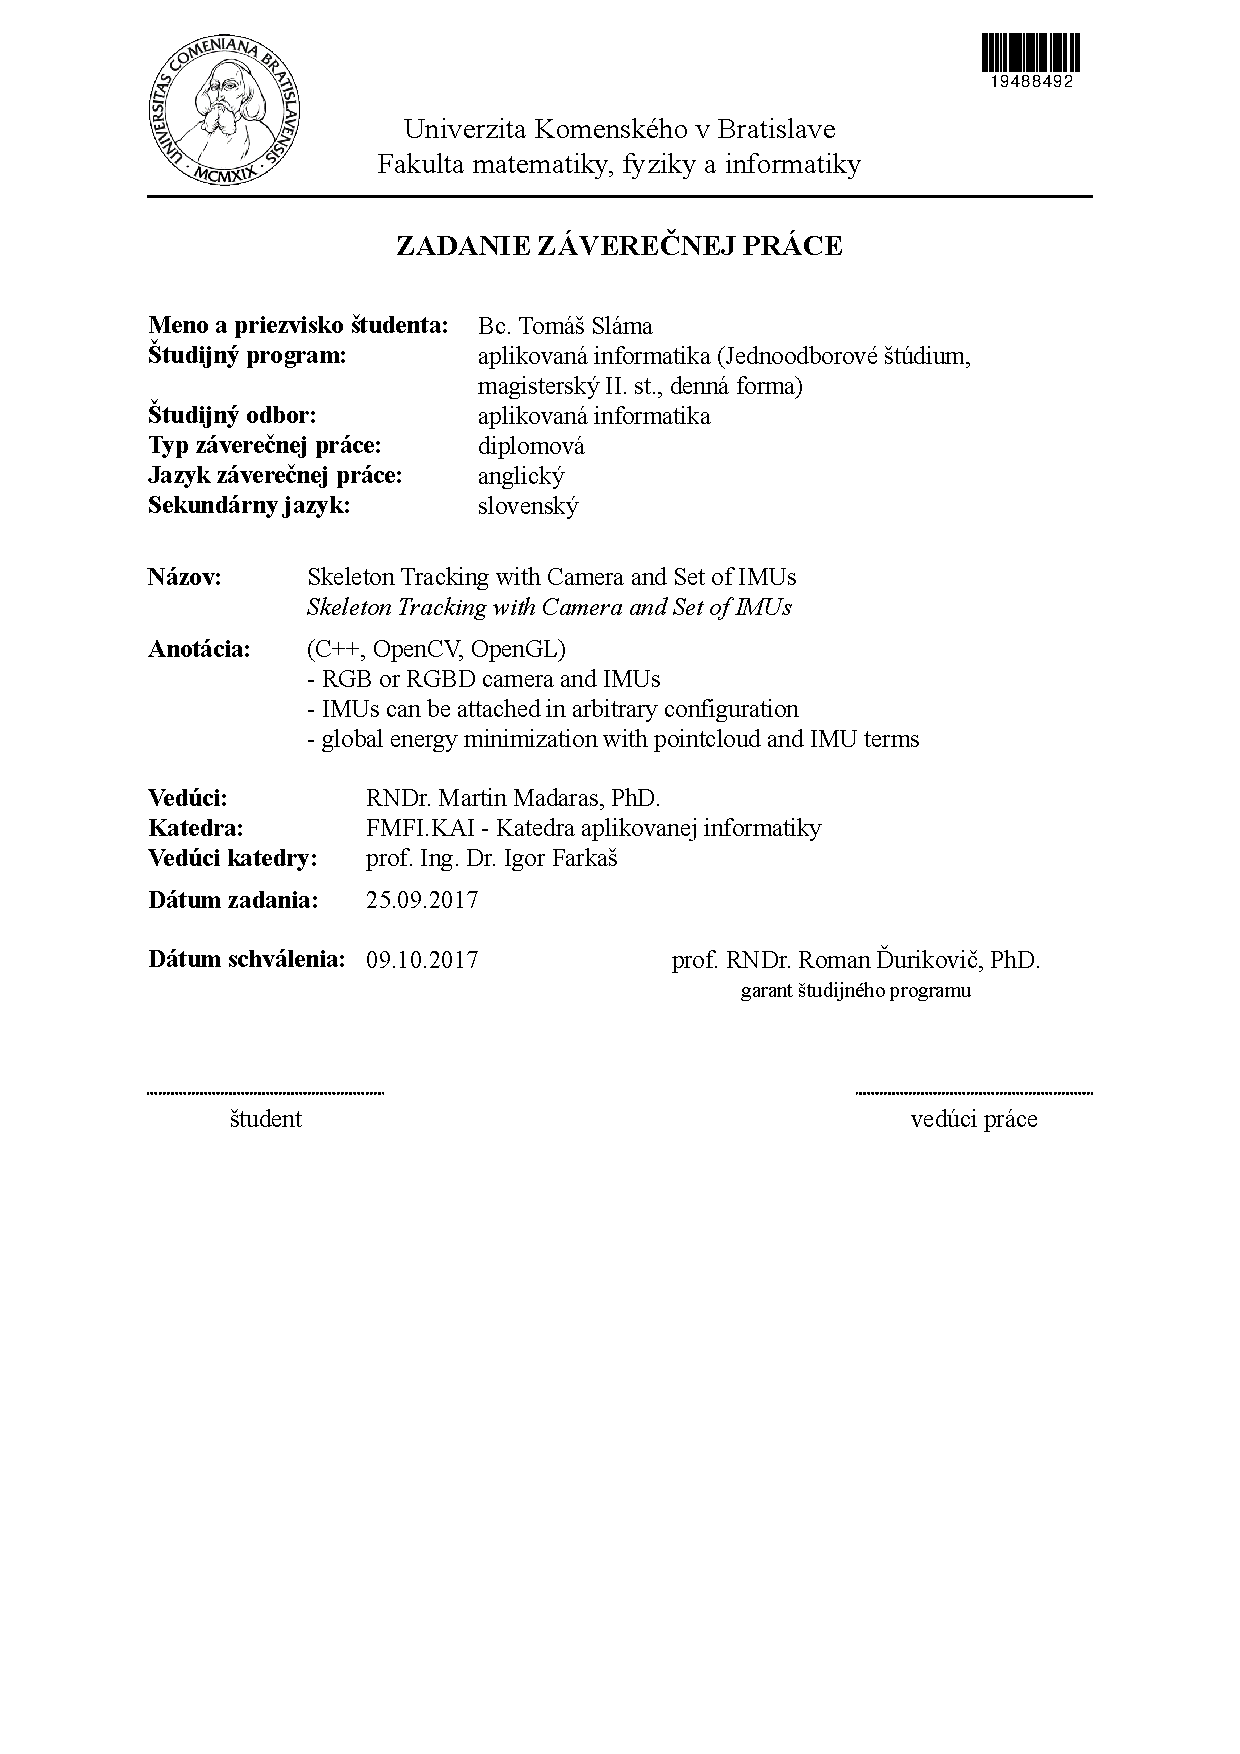
\includegraphics[width=\textwidth]{dip.pdf}


%podakovanie

\flushleft\textbf{\Huge Acknowledgement}\\ \hfill \break
\justify %zarovnanie
I would like to express my grattitude to my supervisor RNDr.  Martin Madaras, PhD. for his guidance and support throughout the elaboration of this thesis.
%koniec podakovania
\setcounter{page}{1}
\newpage

%abstrakt

\flushleft\textbf{\Huge Abstract}\\ \hfill \break
\justify %zarovnanie
	Abstract will be written later \\ \newline
\textbf{\textit{Key words: }}Skeleton, Tracking, Camera, IMU

\newpage

\flushleft\textbf{\Huge Abstrakt}\\ \hfill \break
\justify %zarovnanie
Abstrakt dopisem neskor\\ \newline

\textbf{\textit{Kľúčové slová: }} Skeleton, Tracking, Camera, IMU

\newpage


%koniec abstraktu

\tableofcontents
\listoffigures

\chapter{Prologue}
%\begin{sloppypar}
\section{Introduction}

\justify %zarovnanie

%\end{sloppypar}
%\setcounter{page}{5}
\addcontentsline{toc}{chapter}{\numberline {}Prologue}
Project introduction
%Vychodiska

\subsection{Inspiration}
Recently done projects
\chapter{Theory}
\section{Skeleton tracking}
\section{title}

\begin{thebibliography}{99}

\addcontentsline{toc}{chapter}{\numberline {}Bibliography}

\bibitem{handtracking}
Robust Articulated-ICP for Real-Time Hand Tracking, Ecole Polytechnique Federale de Lausanne (EPFL), Bielefeld University 2015

\bibitem{spheremeshes}
Sphere-Meshes for Real-Time Hand Modeling and Tracking, Anastasia Tkach, Mark Pauly, Andrea Tagliasacchi, 2017

\bibitem{model}
Online Generative Model Personalization for Hand Tracking, ANASTASIA TKACH, ANDREA TAGLIASACCHI, EDOARDO REMELLI, MARK PAULY, ANDREW FITZGIBBON, 2017

\bibitem{mocap}
Optical-Inertial Synchronization of MoCap Suit with Single Camera Setup for Reliable Position Tracking, Adam Riečický, Martin Madaras, Michal Piovarči and Roman Ďurikovič



\end{thebibliography}


\end{document} 


















